\documentclass[12pt,letterpaper]{article}
\usepackage[spanish]{babel}
\usepackage[utf8]{inputenc}
\usepackage{graphicx}
\usepackage{listings}
\usepackage{xcolor}
\usepackage{hyperref}
\usepackage{amsmath}
\usepackage{float}
\usepackage{fancyhdr}
\usepackage{lastpage}
\usepackage{titling}

% Configuración del encabezado y pie de página
\pagestyle{fancy}
\fancyhf{}
\renewcommand{\headrulewidth}{1pt}
\renewcommand{\footrulewidth}{1pt}
\fancyhead[L]{Universidad Católica de Temuco}
\fancyhead[R]{Programación II}
\fancyfoot[C]{Página \thepage\ de \pageref{LastPage}}
\fancyfoot[R]{Octubre 2025}

% Aumentar el espacio superior del título
\setlength{\droptitle}{-4em}

% Configuración de colores y estilo para código
\definecolor{codegreen}{rgb}{0,0.6,0}
\definecolor{codegray}{rgb}{0.5,0.5,0.5}
\definecolor{codepurple}{rgb}{0.58,0,0.82}
\definecolor{backcolour}{rgb}{0.95,0.95,0.92}

\lstdefinestyle{mystyle}{
    backgroundcolor=\color{backcolour},   
    commentstyle=\color{codegreen},
    keywordstyle=\color{magenta},
    numberstyle=\tiny\color{codegray},
    stringstyle=\color{codepurple},
    basicstyle=\ttfamily\footnotesize,
    breakatwhitespace=false,         
    breaklines=true,                 
    captionpos=b,                    
    keepspaces=true,                 
    numbers=left,                    
    numbersep=5pt,                  
    showspaces=false,                
    showstringspaces=false,
    showtabs=false,                  
    tabsize=2
}

\lstset{style=mystyle}

\title{\textbf{Sistema de Gestión de Restaurante}\\
\large Evaluación 2 -- Programación II\\
\vspace{0.5cm}
\normalsize Universidad Católica de Temuco\\
\normalsize Facultad de Ingeniería\\
\normalsize Ingeniería Civil Informática}

\author{
    \textbf{Integrantes:}\\
    \vspace{0.3cm}
    Joaquin Carrasco Duran\\
    \vspace{0.3cm}
    Benjamin Cabrera\\
    \vspace{0.3cm}
    Leonardo Chavez\\
    \vspace{0.3cm}
    \textbf{Profesor:} Guido Mellado\\
    \vspace{0.3cm}
    \textbf{Asignatura:} Programación II\\
    \vspace{0.3cm}
    \textbf{Sección:} 2
}

\date{Octubre 2025}

\begin{document}

\maketitle
\newpage
\tableofcontents
\newpage

\section{Introducción}
Este informe presenta el desarrollo de un sistema de gestión para restaurantes implementado en Python. El sistema permite la administración de inventario, gestión de pedidos, generación de boletas y visualización de menús utilizando una interfaz gráfica moderna con customtkinter.

\section{Objetivos}
\subsection{Objetivo General}
Desarrollar un sistema de gestión integral para restaurantes que permita administrar inventario, pedidos y generación de documentos de manera eficiente.

\subsection{Objetivos Específicos}
\begin{itemize}
    \item Implementar un sistema de gestión de inventario para ingredientes
    \item Crear un sistema de pedidos con interfaz gráfica
    \item Desarrollar un generador de boletas automatizado
    \item Implementar visualización de menús en formato PDF
\end{itemize}

\section{Arquitectura del Sistema}
El sistema está desarrollado siguiendo los principios de la programación orientada a objetos y utiliza varios patrones de diseño para mantener una estructura modular y mantenible.

\subsection{Patrones de Diseño Utilizados}
\begin{itemize}
    \item \textbf{Patrón Facade}: Implementado en la clase BoletaFacade para simplificar la generación de boletas.
    \item \textbf{Patrón Interface}: Utilizado en IMenu para definir el contrato de los elementos del menú.
    \item \textbf{Patrón Composite}: Aplicado en la estructura de menús e ingredientes.
\end{itemize}

\section{Diagrama de Clases}
\subsection{Estructura del Sistema}
\begin{figure}[H]
    \centering
    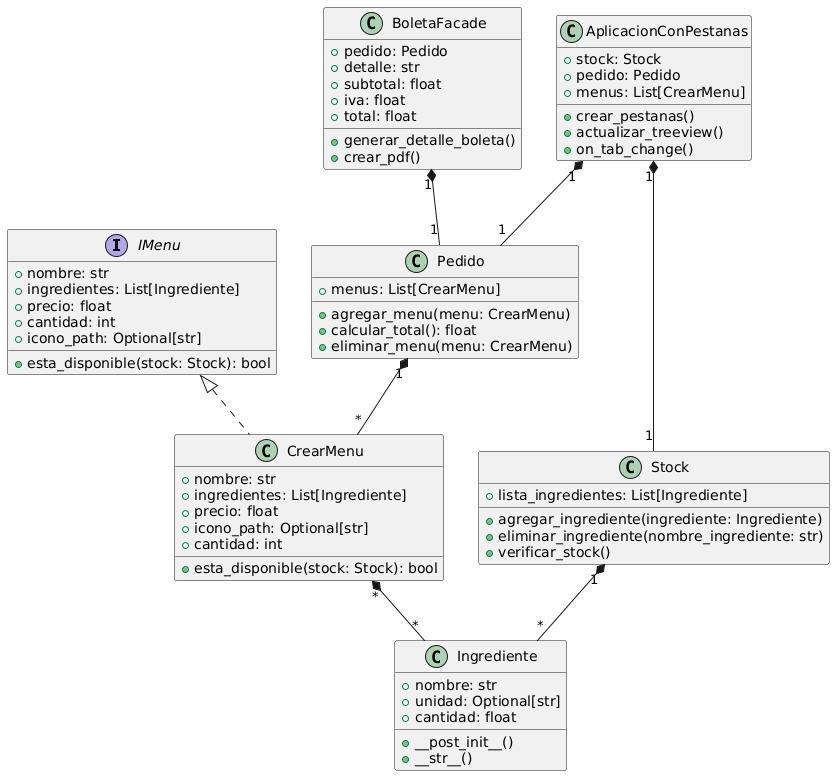
\includegraphics[width=\textwidth]{./images/diagrama.png}
    \caption{Diagrama de Clases del Sistema}
    \label{fig:diagrama}
\end{figure}

\subsection{Explicación del Diagrama}
\begin{figure}[H]
    \centering
    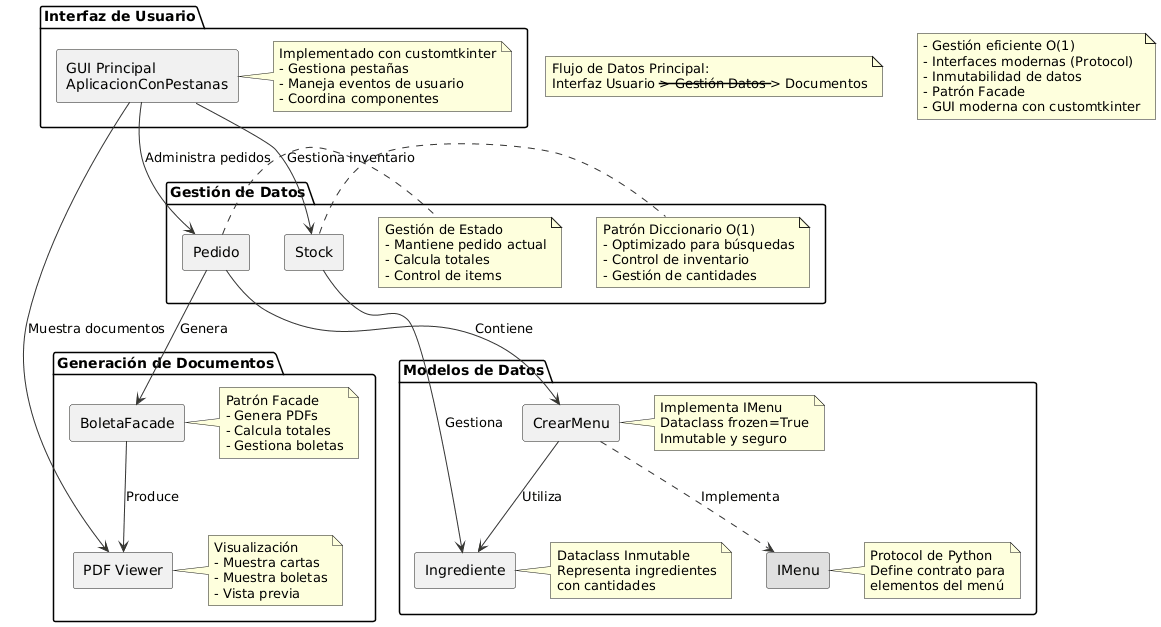
\includegraphics[width=\textwidth]{./images/explicacion_diagrama.png}
    \caption{Explicación Detallada de las Relaciones entre Clases}
    \label{fig:explicacion-diagrama}
\end{figure}

\subsection{Descripción de las Clases}
\begin{itemize}
    \item \textbf{AplicacionConPestanas}: Clase principal que coordina todas las funcionalidades del sistema.
    \item \textbf{Stock}: Gestiona el inventario de ingredientes.
    \item \textbf{Ingrediente}: Representa los ingredientes individuales.
    \item \textbf{CrearMenu}: Implementa la interfaz IMenu y representa los elementos del menú.
    \item \textbf{Pedido}: Maneja la gestión de pedidos.
    \item \textbf{BoletaFacade}: Simplifica la generación de boletas.
\end{itemize}

\section{Implementación}
\subsection{Gestión de Inventario}
El sistema maneja el inventario a través de la clase Stock, que permite:
\begin{itemize}
    \item Agregar nuevos ingredientes
    \item Eliminar ingredientes existentes
    \item Verificar disponibilidad
    \item Actualizar cantidades
\end{itemize}

\subsection{Sistema de Pedidos}
La gestión de pedidos se realiza mediante la clase Pedido, que ofrece:
\begin{itemize}
    \item Agregar elementos al pedido
    \item Calcular totales
    \item Verificar disponibilidad de ingredientes
    \item Generar boletas
\end{itemize}

\section{Interfaz Gráfica}
El sistema utiliza customtkinter para crear una interfaz gráfica moderna y amigable que incluye:
\begin{itemize}
    \item Pestañas para diferentes funcionalidades
    \item Visualización de menús con imágenes
    \item Visor de PDF integrado
    \item Formularios para gestión de inventario
\end{itemize}

\section{Conclusiones}
El sistema desarrollado cumple con los objetivos planteados, proporcionando una solución integral para la gestión de restaurantes. La implementación de patrones de diseño y principios de programación orientada a objetos permite una estructura mantenible y extensible.

\section{Anexos}
\subsection{Código Fuente}
A continuación se presentan fragmentos relevantes del código:

\begin{lstlisting}[language=Python, caption=Implementación de BoletaFacade]
class BoletaFacade:
    def __init__(self, pedido):
        self.pedido = pedido
        self.detalle = ""
        self.subtotal = 0
        self.iva = 0
        self.total = 0

    def generar_detalle_boleta(self):
        self.detalle = ""
        for item in self.pedido.menus:
            subtotal = item.precio * item.cantidad
            self.detalle += f"{item.nombre:<30} {item.cantidad:<10} ${item.precio:<10.2f} ${subtotal:<10.2f}\n"
        
        self.subtotal = self.pedido.calcular_total()
        self.iva = self.subtotal * 0.19
        self.total = self.subtotal + self.iva
\end{lstlisting}

\end{document}